\documentclass[a4paper, 12pt]{article}

\usepackage[left = 3cm, top = 3cm, bottom = 3cm, right = 2cm]{geometry}
\usepackage{graphicx}
\usepackage[spanish,es-tabla]{babel} % Idioma español con tablas
\usepackage{amsmath}
\usepackage{amssymb}
\usepackage{amsfonts}
\usepackage[utf8]{inputenc}         % Para escribir en castellano
\usepackage[T1]{fontenc}
\usepackage{color}
\usepackage{alltt}
\usepackage{times}
\usepackage{setspace}  % Usado para doble espacio, espacio y medio y espacio simple
\usepackage{booktabs}         % Para formar tablas
%\usepackage{longtable}       % Usado para diseñar grandes tablas.
\usepackage[round]{natbib} 
\bibliographystyle{apalike}


\begin{document}

\begin{center}
 {\bf {\fontsize{14}{16.8}\selectfont UNIVERSIDAD NACIONAL DE TRUJILLO}}     
 
    {\bf{\fontsize{14}{16.8}\selectfont Facultad de Ciencias físicas y matemáticas}} 

  {\bf{\fontsize{14}{16.8}\selectfont Escuela Académico Profesional de Informática}}
\end{center}  

\begin{figure}[ht]
\begin{center}

\includegraphics[width=.3\textwidth]{unt}
\end{center}
\end{figure}
\vskip 1cm
\begin{center}
  { \bf {\fontsize{17}{20.4}\selectfont{RECONOCIMIENTO AUTOMÁTICO DE SEÑALES DE TRÁNSITO MEDIANTE PROCESAMIENTO DE IMÁGENES Y RED NEURONAL PERCEPTRÓN MULTICAPA}}  } 
\end{center}   
  \vskip 1cm
  { \bf {\fontsize{17}{20.4}\selectfont{\hspace*{-0.4cm}Nombre de autor(es): }}  } 
  \vskip 1cm
  { \bf {\fontsize{17}{20.4}\selectfont{\hspace*{4cm}Polo Cosme Juan Diego }}  } 
  \vskip 1cm
  { \bf {\fontsize{17}{20.4}\selectfont{\hspace*{4cm}Sanchez Chavez Marlon Dennis }}  } 
  \vskip 1cm
  { \bf {\fontsize{17}{20.4}\selectfont{\hspace*{-1cm}Nombre del Asesor: }}  }
  \vskip 1cm
  { \bf {\fontsize{17}{20.4}\selectfont{\hspace*{4cm}Gutierrez Gutierrez Jorge }}  } 
\vskip 4cm
\begin{center}    
{\bf {\fontsize{14}{16.8}\selectfont Trujillo - La Libertad
\vskip 0.0cm
\hspace*{-0.2cm} 
2017 }}
\end{center} 
\newpage

\begin{center}
%\onehalfspace  \doublespacing  \singlespace
\Large {PROYECTO DE INVESTIGACIÓN PARA TRABAJO DE GRADUACIÓN \\
\vskip 0.2cm
 ESCUELA ACADÉMICO PROFESIONAL DE INFORMÁTICA}
\end{center}
\vskip 1cm

\section{GENERALIDADES}

\subsection{Título}
Reconocimiento Automático de señales de tránsito mediante procesamiento de imágenes y red neuronal perceptrón multicapa.
\subsection{Autores}
\begin{center}
\begin{table}[h!]
\centering
%\caption{Datos del alumno (s) investigador (es)}
\begin{tabular}{llrrrr} \toprule
Código(s) & Nombres y Apellidos& Cargo en el proyecto&Email \\ \midrule
10127001-13 & Juan Polo Cosme & Estudiante invest. & juan.diego.al@hotmail.com           \\
10527003-13 & Marlon Sanchez Chavez & Estudiante invest. & marlon.sanchez.chavez@gmail.com            \\ \bottomrule
\end{tabular}
\end{table}
\end{center}



\subsection{Tipo de investigación}
\subsubsection{De acuerdo al fin que se persigue (Básica/Aplicada):} Aplicada
\subsubsection{De acuerdo al diseño de investigación (Descriptiva / Explicativa):} Descriptiva



\subsection{Área y línea de Investigación}
\subsubsection{Área de investigación :} Sistemas Inteligentes 
\subsubsection{Línea de Investigación:} Machine Learning
\subsubsection{Tema de investigación :} Redes Neuronales


\subsection{Localidad e Institución donde se desarrollará el proyecto }
  
\subsubsection{Localidad (Dirección, Distrito, Provincia, Departamento) :} Jr. 20 de Junio 1673 , Florencia de mora , Trujillo , La Libertad 
\subsubsection{Institución (Universidad/Facultad/Departamento):} Universidad Nacional de Trujillo , Facultad de Ciencias Fisicas y Matematicas , Departamento de Informática

  
\subsection{Duración del trabajo de graduación (Plan TG y desarrollo del TG)}
\hspace*{0.7cm}Del \hspace*{0.2cm}20/08/2017 \hspace*{0.3cm} AL\hspace*{0.2cm}15/01/2018  \hspace*{0.2cm}(4 meses y 25 días)
  
    
  
  
\subsection{Cronograma del trabajo de graduación}


\subsubsection{Cronograma del plan TG y avance del desarrollo TG }

 \begin{table}[h!]
\centering
\begin{tabular}{|p{3cm} |p{4cm} |p{2.2cm} |p{2.6cm} |p{2.3cm}|} \hline
\textit{{\bf{Etapas}}} & \textit{{\bf{Actividades/tareas}}} & \textit{{\bf{Fecha inicio}}} & \textit{{\bf{Fecha término}}} & \textit{{\bf{Hs. semanal}}}\\ \hline

Preparación del plan TG & Elaborar plan TG.\par Aprob. plan GT por jurado.  & 20/08/2017\par 26/09/2017 & 26/09/2017\par 21/10/2017 & 15\par 10  \\ \hline
Recolección de datos & Inv. bibliográfica.\par Instrumentos de medición. & 22/10/2017\vskip 0.5cm \par 30/10/2017  & 29/10/2017\vskip 0.5cm \par 15/11/2017 & 30\vskip 0.5cm\par 25    \\  \hline

Análisis de resultados & Preparar resultados  preliminares. &\vskip 0.2cm 16/11/2017 &\vskip 0.2cm 29/11/2017 & \vskip 0.2cm 50 \\ \hline
Redacción del informe  &Planteamiento, marco teórico y metodología.\par Informe I: Avance TG. \par
Resultados y conclusiones.\par Informe II: Avance TG. &\vskip 0.2cm\par 30/11/2017\par 20/12/2017 \vskip 0.6cm\par 21/12/2017\par 15/01/2018 & \vskip 0.2cm\par 19/12/2017\par 20/12/2017 \vskip 0.6cm\par 14/01/2017\par 15/01/2018 &  
\vskip 0.2cm\par 30\par 10 \vskip 0.6cm\par 40\par 10                \\  \hline
\end{tabular}
\end{table}


\subsubsection{Cronograma de trabajo de graduación (Plan TG y desarrollo del TG)}

 \begin{table}[h!]
\centering
\begin{tabular}{|p{3.9cm} |p{5.6cm} |p{2.1cm} |p{2.1cm} |p{1.5cm}|} \hline
\textit{{\bf{Etapas}}} & \textit{{\bf{Actividades/tareas}}} & \textit{{\bf{Fecha inicio}}} & \textit{{\bf{Fecha término}}} & \textit{{\bf{Horas semanal}}}\\ \hline
Recolección de datos & Redacción del plan de Tesis \par Revisión Bibliográfica\par Elaboración del marco teórico  & \par 20/08/2017\par \par 18/10/2017\par 02/11/2017     & 16/10/2017\par 01/11/2017\par 10/12/2017       & 20\par 20\par 20                 \\  \hline
Análisis de resultados & Implementar Sistema clasificador \par Contrastación de Hipótesis\par Discusión de resultados  &   01/01/2018\par 22/02/2018\par 23/03/2018   &  21/02/2018\par 22/03/2018\par 23/04/2018    &              
30\par 30\par 30  \\  \hline
Redacción del informe  & Presentar Informe  &  24/04/2018    &  05/05/2018    &        20          \\  \hline
\end{tabular}
\end{table}

\newpage


\subsection{Recursos disponibles}
\subsubsection{{\bf Personal:}} 
Investigador 1 : Juan Polo Cosme \vskip 0.1cm
Investigador 2 : Marlon Sanchez Chavez \vskip 0.1cm
Asesor : Jorge Gutierrez Gutierrez
\subsubsection{ {\bf	Materiales y Equipos:}} 
Laptop Toshiba (cantidad = 2).\vskip 0.1cm
Cámara - Canon Powershot SX610 HS (cantidad = 1).\vskip 0.1cm
Memoria USB(cantidad=1)\vskip 0.1cm
Hojas Bond(cantidad= 1 ciento)\vskip 0.1cm
Lapices(cantidad=2)\vskip 0.1cm
Lapiceros(cantidad=6)\vskip 0.1cm
\subsubsection{{\bf Locales:}} 
Domicilio : 20 de Junio 1673 - Florencia de Mora - Trujillo - La Libertad \vskip 0.1cm
Universidad : Av. Juan Pablo II cuadra 3 - Trujillo - La Libertad

\subsection{Presupuesto}

\subsubsection{Bienes}

\begin{enumerate}
\item[1.-]Cámara - Canon Poweshot SX610 HS \vskip 0.3cm
\begin{enumerate}
\item[a)] Total : 109.50 soles
\vskip 0.3cm
\end{enumerate}
\end{enumerate}


\subsubsection{Servicios}

\begin{enumerate}

\item[1.-]Movilidad
\begin{enumerate}
\item[a)] Total : 6 soles semanales
\vskip 0.3cm
\end{enumerate}

\item[2.-]Internet 8MB
\begin{enumerate}
\item[a)] Total : 80 soles mensual
\vskip 0.3cm
\end{enumerate}

\item[3.-]Impresiones
\begin{enumerate}
\item[a)] Total : 2 soles semanal
\vskip 0.3cm
\end{enumerate}

\item[4.-]Memoria USB
\begin{enumerate}
\item[a)] Total : 30 soles 
\vskip 0.3cm
\end{enumerate}

\item[5.-]Folder Manila
\begin{enumerate}
\item[a)] Total : 0.50 soles semanal 
\vskip 0.3cm
\end{enumerate}

\item[6.-]Desayuno y Almuerzo
\begin{enumerate}
\item[a)] Total : 20 soles semanal 
\vskip 0.3cm
\end{enumerate}

\item[7.-]Útiles de Oficina (Hojas bond , lápiz , lapiceros)
\begin{enumerate}
\item[a)] Total : 10 soles
\vskip 0.3cm
\end{enumerate}

\end{enumerate}

\subsubsection{Resumen de presupuesto}
\begin{center}
\begin{table}[h!]
\centering
\begin{tabular}{llrrrr} \toprule
Rubro & Importe \\ \midrule
Bienes & S/. 109.50      \\
Servicios & S/. 300.00           \\ \bottomrule
Total & S/. 409.50
\end{tabular}
\end{table}
\end{center}

\subsection{Financiamiento}
\subsubsection{ {\bf	Con recursos universitarios:}}  No contamos con recursos universitarios.
\subsubsection{ {\bf Con recursos externos:}} No contamos con recursos externos.
\subsubsection{ {\bf Autofinanciación:}} Contamos con recursos autofinanciados para solventar los bienes y servicios usados en la elaboración del trabajo de investigación. Aproximadamente de 60 soles mensual cada investigador .

\subsection{Resumen del proyecto}
El presente proyecto estudia el problema de la no detección inmediata de señales de tránsito que son muchas veces la causa de diferentes tipos de accidentes de tránsito y por ende la muerte de muchas personas. Muchas veces se dan por negligencia de los conductores o los mismos peatones ya sea que estuvo distraído o simplemente no quiso respetar las señales teniendo como objetivo implementar un software de reconocimiento automático de señales de tránsito que le avise al usuario que una señal fue detectada , así mismo que también informe que tipo de señal es.\par
\vskip 0.6cm
Para lo cual se va a utilizar  algoritmos de procesamiento de imágenes  tales como segmentación,SURF, binarización , reducción , ampliación ,etc; y el diseño , entrenamiento(por medio del algoritmo back propagation ) de las redes neuronales perceptrón multicapa para la clasificación de la señal.También se utilizará el lenguaje de programación Java(el ide usado es Netbeans) con la librería gráfica Open CV y la herramienta Joone para el tema de la red neuronal.\par
\vskip 0.6cm
Se espera obtener un software eficiente y eficaz , reduciendo el margen de error en mínimo 2 puntos con respecto a anteriores trabajos , y que sea capaz de ser utilizado por diferentes tipos de usuarios sin ningún inconveniente.\par
\vskip 0.6cm
En conclusión, el uso de una red neuronal reduce considerablemente el error y el tiempo en la clasificación de imágenes.\par


\newpage

\section{PLAN DE INVESTIGACIÓN}

\subsection{Antecedentes}

\citep{sirlopu2016deteccion} Se estudia la detección de caries en las placas radiográficas utilizando procesamiento de imágenes.El proceso consistió en una etapa de pre procesamiento para eliminar el ruido aplicándole filtros(Blur,Gaussian Blur , Median Blur,Histograma) para suavizar la imagen.En la segunda fase realiza la etapa de procesamiento segmentando la imagen por medio del método de binarización y el método Otsu.La tercera fase consiste en la extracción de características de las imágenes procesadas utilizando una herramienta de visión artificial llamada Balu Tolbox que sirve para extraer las características de las imágenes.La cuarta etapa es la de clasificación donde utilizo dos clasificadores : Una red neuronal perceptrón multicapa y Naive Bayes que es un clasificador probabilístico.Llegamos a la conclusión que los diferentes métodos usados para el pre procesamiento y procesamiento de imágenes digitales en esta tesis puede ser adaptado para nuestro software a desarrollar.\par


\vskip 1cm

\citep{mundaca2016deteccion} Trata sobre el reconocer automáticamente las placas de automóviles.El proceso consistió en una etapa de pre procesamiento cambiando la imagen a escala de grises y localizando la placa mediante la ubicación de concentración de gradientes. En la segunda fase corrigió la perspectiva de la imagen si en caso es necesario para tenerla de manera frontal utilizando la transformada de Hough.La tercera fase consiste en la segmentación de la imagen haciendo un recorte horizontal y uno vertical para  solo obtener los números de la placa.La cuarta etapa es la reducción de la imagen a la dimension de las plantillas que tiene almacenadas de los caracteres de las placas.La quinta etapa consiste en comparar las matrices de la plantilla y la imagen de entrada para obtener el carácter que representa.Llegamos a la conclusión que el método de localización , de corrección de perspectiva , de segmentación y de reducción de la imagen pueden ser adaptados para nuestro software a desarrollar.\par


\vskip 1cm
\citep{caiza2016diseno} Presenta el diseño de una aplicación interactiva que permita asistir al conductor en el reconocimiento de señales de tránsito en la vía, mediante procesamiento de imágenes, utilizando software libre y tecnología BEAGLEBONE.El proceso consistió primero en la creación de una base de datos almacenando las diferentes señales de tránsito que existen.En la segunda fase se compara la imagen de entrada con las imágenes de las señales almacenadas mediante los puntos característicos que brinda el algoritmo surf para cada imagen.a tercera fase consiste en implantar el programa en una tarjeta beaglebone para avisar de manera sonora si la señal fue encontrada.Llegamos a la conclusión que el algoritmo surf es muy potente para el reconocimiento de un objeto y que puede ser adaptado para nuestro software a desarrollar.\par


\vskip 1cm

\citep{ChavezAlex} Determina la presencia, ubicación y orientación de los vehículos que desean ingresar a una avenida de alto tráfico y doble sentido, desde una vía secundaria en una intersección de tipo 'T' .El proceso de pre procesamiento consistió en pasar la imagen a escala de grises y ajustar la resolución de la imagen a 320x240 px.En la segunda fase se compara la imagen entrante con la plantilla que se tiene de la misma calle para observar los cambios producidos ya que esos serán los autos que se encuentran en ese momento.La tercera fase consiste utilizar diferentes filtros de procesamiento (Umbralizacion ,Enmascaramiento, Filtro Mediana) para solo obtener como resultado los autos en ese momento.La cuarta fase sirve para analizar el numero de vehículos que hay y las características de estos (ubicación,dimensiones y orientación), para eso se aplica segmentación y una función llamada orientación.Llegamos a la conclusión que la umbralizacion , el enmascaramiento y el filtro mediana sirven de manera eficiente para eliminar el ruido y solo obtener la región de trabajo que necesitamos y que dichos métodos son adaptables a nuestro software a desarrollar.\par

\vskip 1cm
\citep{salazar2015desarrollo} Desarrolla un algoritmo que permita obtener la localización de la región de la placa vehicular peruana en una imagen digital, usando métodos y técnicas de procesamiento de imágenes.El proceso de pre procesamiento consistió en pasar la imagen a escala de grises.En la segunda fase se aplica la umbralización en la imagen de entrada para eliminar el ruido .La tercera fase consiste en binarizar la imagen de entrada para un procesamiento adecuado.La cuarta fase consiste en formar todos los cuadros posibles existentes en la imagen de entrada, obteniendo varias posibles candidatas de placa.La quinta fase consiste seleccionar la placa correcta y aplicarle un filtro final.Llegamos a la conclusión que el algoritmo de obtener posibles cuadrados candidatos es adaptable para nuestro software a desarrollar.\par


\vskip 1cm
\citep{ayunque} Reconoce señales de tránsito usando una red neuronal convolucional, la cual usa varias capas, las principales son convolución y reducción de muestreo, donde cada capa recibe un dato de entrada en 3 dimensiones (ancho, alto y profundidad) que es trasformado en dato de salida en 3 dimensiones diferentes. La red neuronal aprende filtros que se activan cuando observa un cierto borde o contorno en una orientación especifica.Usa backpropagation para entrenar a la red neuronal.
De tal manera, en nuestra propuesta decidimos optar por una red neuronal perceptrón multicapa, entrenándola con backpropagation, de tal manera que podamos mejorar el porcentaje de acierto, y poder clasificar una señal de tránsito.\par


\vskip 1cm
\citep{diazrojas} Reconoce las placas de un automóvil usando un perceptron multicapa, donde la red neuronal fue entrenada con backpropagation, y para el reconocimiento de los números y letras, hace segmentaciones donde solo quede la letra o numero para luego clasificarla, cada letra o número sea convertida a matriz para que cada dígito de 0 o 1, sea una entrada para la red.
En nuestro modelo propuesto, usaremos la segmentación para preparar la imagen, convertiremos la imagen de tal forma que pueda ser convertida a matriz de 0 y 1, para luego ser pasada como entradas a la red neuronal.\par

\vskip 1cm
\citep{carranzahernandez} cuyo objetivo es reconocer caracteres dibujados a mano, usando el método de aprendizaje resilient backpropagation, teniendo pesos y bias para la red neuronal, luego hace muchos testeos para saber cuan efectivo ha sido el proceso de entrenamiento del sistema de red neuronal.
En nuestra propuesta hemos decidido hacer nuestra fase de pruebas o testeo, para saber la afectividad de acierto del reconocedor. Volviendo a entrenar los pesos y bias hasta tener un mínimo porcentaje de error.\par

\vskip 1cm
\citep{camposaquino} Reconoce el melanoma humano para detectar si es maligno o benigno, en esta tesis el autor sigue los mismos pasos de reconocimiento y procesamiento de imagen, pero para este tema, es importante tomar en cuenta el color, ya que las manchas en la piel definen si es cancerígeno o no, entonces toma lo que es el espacio de color, como el RGB y el HSV.
Nosotros en nuestra propuesta obviamos el color ya que vamos a detectar señales de tránsito tipo prevención y estas tienen un color en común, entonces vamos a trabajarla de blanco y negro.\par

\vskip 1cm
\citep{arriagaGarcia} Reconoce las señales de tránsito, los autores emplean un algoritmo llamado matching de Chamfer para realizar la detección de bordes, esto agiliza el procesamiento de entradas para la red neuronal.
Para nuestra propuesta pensamos también generar bordes, pero preferimos optar por algoritmos de OpenCV ya que también prepara la imagen para generar una matriz y poder reconocerla mediante nuestro Perceptrón multicapa.\par


\subsection{Fundamentación científica, técnica o humanística}

\subsubsection{Señales de Tránsito}
\begin{enumerate}
\item[1)]Definición
\vskip 0.3cm
Según \cite{dextre2012senalizacion} La señalización es un lenguaje especial para comunicar ciertos mensajes a los usuarios que transitan por la vía(Ver Figura 1).Donde:\par
- El emisor es el elemento donde está aplicado el signo.\par
- El mensaje es el significado de la señal.\par
- El receptor es el usuario (automovilista,peatón,ciclista,etc.).\par
La señalización no es un simple adorno de la vía ,sino que cumple las siguientes funciones  fundamentales:\par
- Organiza el tránsito\par
- Advierte los peligros\par
- Ordena conductas de seguridad\par
- Comunica informaciones útiles\par
\begin{figure}[ht]
\begin{center}
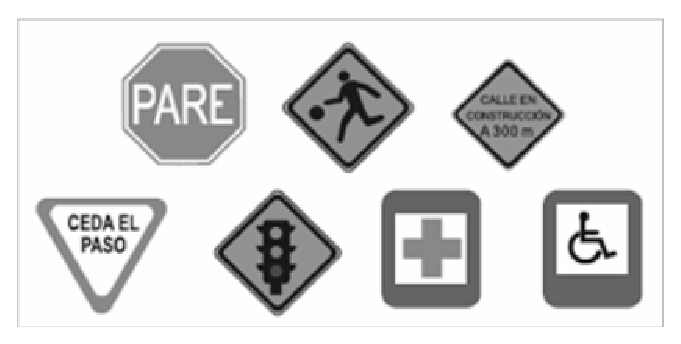
\includegraphics[width=0.4\textwidth]{definicion_senal}
\end{center}
\begin{center}
\caption{\small{Algunas señales de tránsito}}
{\small{Fuente : \cite{dextre2012senalizacion}}}
\end{center}
\end{figure}

\vskip 4cm

Según \cite{caiza2016diseno} Las señales de tránsito son imágenes, letras y números de diferentes colores, tamaños y formas que se ubican en carteles en la vía pública, cuya simbología tienen un significado para  alertar al peatón o conductor a tomar “precauciones” o alertar de las situaciones que se dan en la carretera y vía pública.\par
Tipos :\par
- Informativas \par
Las “señales informativas”  tienen como finalidad servir de guía y encaminar al conductor en la vía sobre sitios de interés, de esta manera las señales de tránsito para el conductor se convierte en objetos muy útiles para su normal traslado y arribo  al destino. Son  “carteles de forma rectangular, de fondo verde y letras blancas o fondo azul y letras blancas”.  \par
- Preventivas \par
Las “señales preventivas” advierten a los conductores de la “presencia de riesgos en la vía”, siendo los peligros por causa de la geografía y de condiciones naturales. Los carteles tienen “forma de  rombo, de fondo amarillo y los símbolos de color negro”, por lo general son las que con más frecuencia se las localiza en las carreteras(Ver Figura 2).\par
\begin{figure}[ht]
\begin{center}
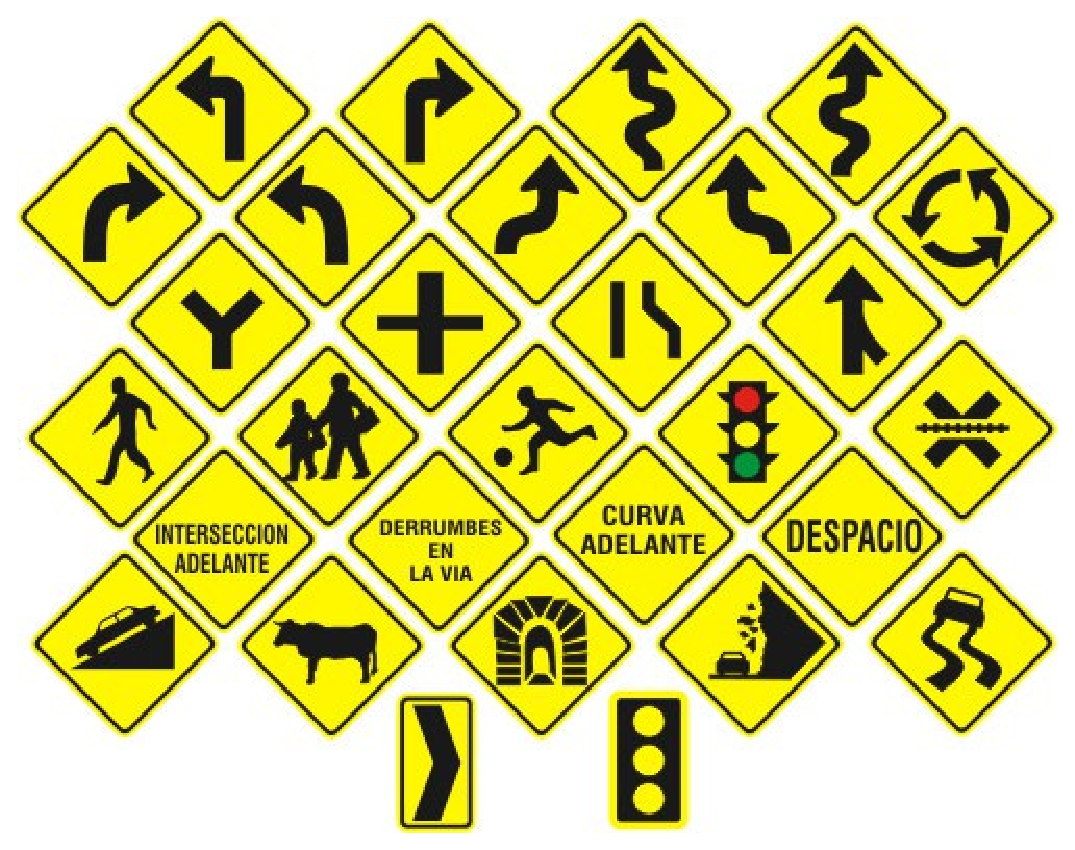
\includegraphics[width=0.5\textwidth]{senales_preventivas}
\end{center}
\begin{center}
\caption{\small{Señales de tránsito preventivas}}
{\small{Fuente : Elaboracion Propia}}
\end{center}
\end{figure}

- Prohibitivas y Reguladores \par 
Son utilizadas para “alertar” a los conductores sobre la “existencia de limitaciones, prohibiciones y restricciones” en la carretera y  vía pública. Los carteles tienen “forma rectangular con fondo blanco y letras en color rojo y negro”. Las señales de tránsito se alinean de manera vertical u horizontal, las señales que están montadas en placas y se colocan en postes son de señalización vertical y las señales de  palabras, símbolos y objetos que se sitúan sobre el pavimento son de señalización horizontal.\par
\vskip 3cm
El presente proyecto se centrará en la señales de tránsito preventivas puesto que el objetivo primordial es prevenir a los conductores para evitar posibles accidentes y muertes a causa de ese motivo.\par
\end{enumerate}

\subsubsection{Pre-Procesamiento de Imágenes}
El preprocesamiento de imágenes es la etapa donde se prepara la imagen para poder obtener en la siguiente etapa el vector de caracteristicas, basicamente elimina las areas que no serviran quedandose solo con el area de trabajo ; tambien en esta etapa se elimina el ruido , se corrige la imagen de acuerdo a los fines que se necesita.\par
\begin{enumerate}
\item[1)] Algoritmo SURF
\vskip 0.3cm
Desarrollado por Herbert Bay, como un detector y descriptor de puntos de interés para el reconocimiento de objetos. Se considera una evolución del algoritmo SIFT. Siendo una de sus ventajas sobre otros métodos, el mejoramiento de la velocidad de cálculo y la robustez ante transformaciones de las imágenes. Estas mejoras se consiguen mediante la reducción de la dimensión y complejidad en el cálculo de los vectores de características de los puntos de interés obtenidos, mientras continúan siendo suficientemente particulares e igualmente repetitivos. El algoritmo SURF consta de tres etapas y se muestran a continuación de manera detallada.\citep{caiza2016diseno} \par

Básicamente este algoritmo consiste en encontrar puntos de interés de las imágenes , asignar la orientación de la región de trabajo de la imagen y extraer esos puntos de interes como una matriz de descriptores.\par
En este proyecto el algoritmo Surf servirá para encontrar de las imágenes tomadas en tiempo real la región donde se encuentra las señales de tránsito .\par
\begin{figure}[ht]
\begin{center}
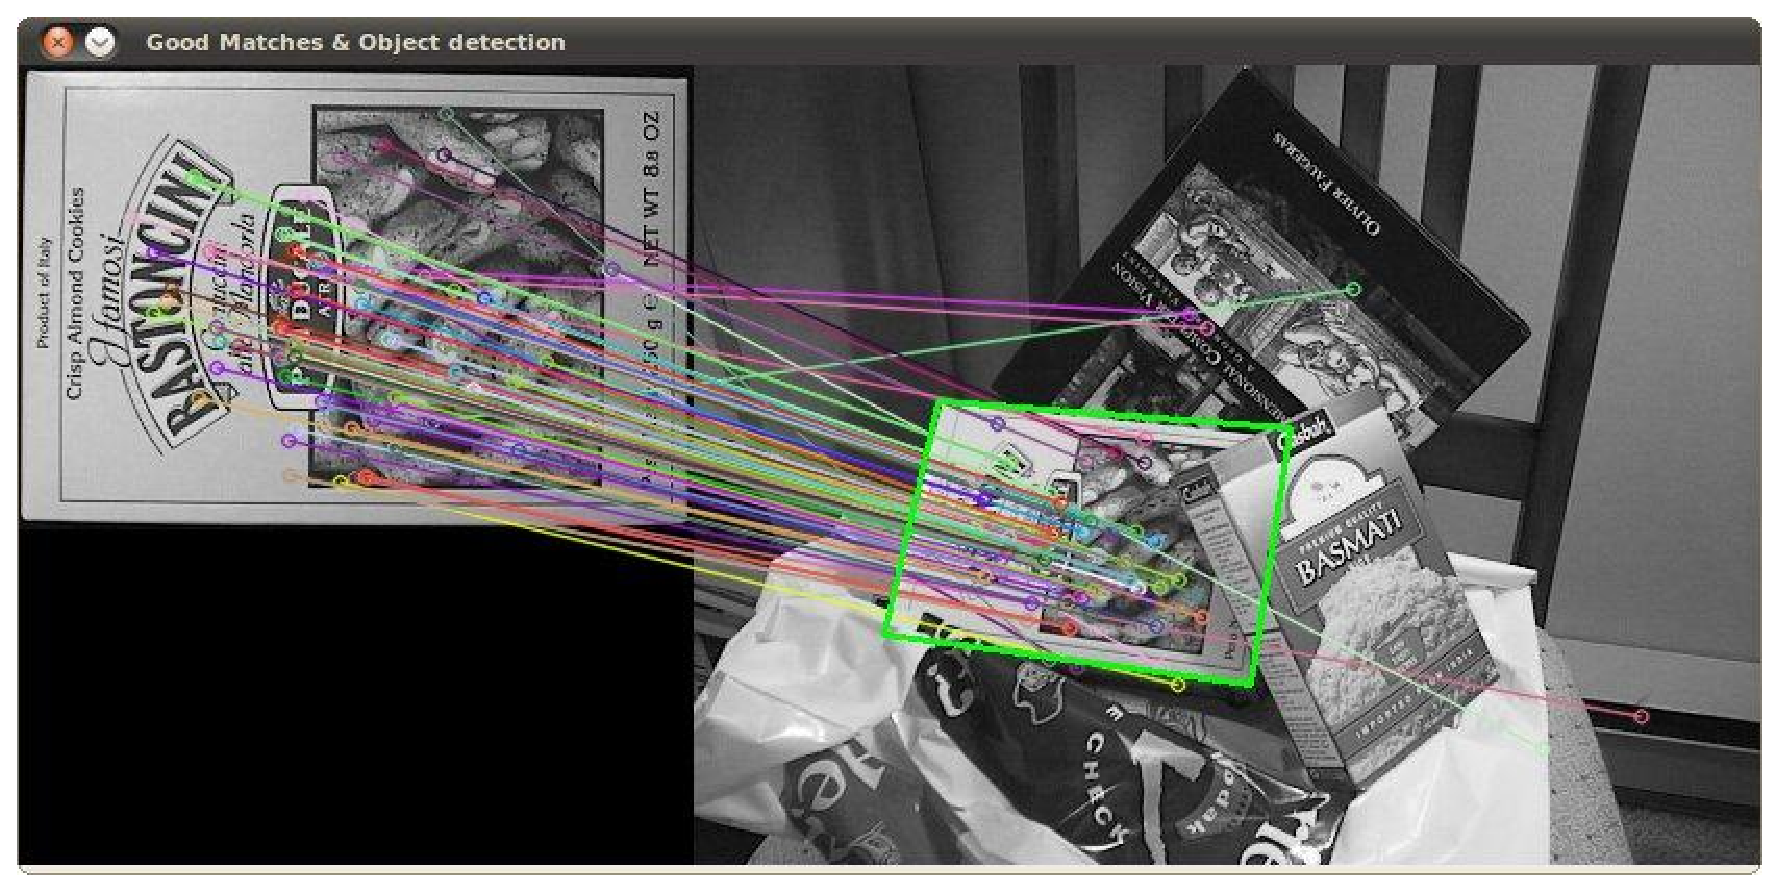
\includegraphics[width=0.5\textwidth]{surf}
\end{center}
\begin{center}
\caption{\small{Detección con el algoritmo SURF}}
{\small{Fuente : Elaboración Propia}}
\end{center}
\end{figure}
\vskip 0.3cm

Como podemos observar en la Figura 3 en la parte izquierda tenemos la imagen base donde sus puntos de interés ya fueron extraídos y almacenados en una base de datos como tipo BLOB  , en la parte derecha se encuentra la imagen tomada en tiempo real para buscar sus puntos de interes y compararlos con los puntos de interés de la imagen base.En conclusión , se puede observar que el algoritmo SURF detecta eficientemente una imagen base sin importar la orientación ni tampoco el tamaño.

\vskip 0.3cm

\item[2)] Segmentación de Imágenes
\vskip 0.3cm
La segmentación subdivide una imagen en sus partes constituyentes u objetos, con el fin de separar las partes de interés del resto de la imagen, por lo tanto el nivel al que se lleva a cabo esta subdivisión depende del problema a resolver. \citep{palomino2009tecnicas} \par
La segmentación automática es una de las tareas más difíciles del procesamiento de imágenes, esta etapa determina el eventual éxito o fracaso del análisis, de hecho rara vez llega a alcanzar una solución satisfactoria,se debe buscar un método alternativo de comprobación para la verificación de los resultados. Un considerable número de trabajos de investigación se centran en este problema.\citep{palomino2009tecnicas} \par

\begin{figure}[ht]
\begin{center}
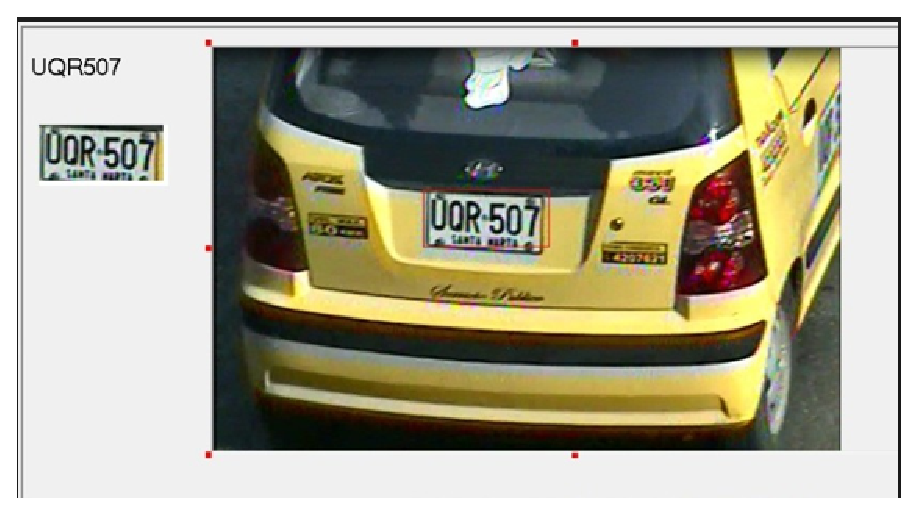
\includegraphics[width=0.5\textwidth]{segmentacion}
\end{center}
\begin{center}
\caption{\small{Proceso de segmentación de una placa de auto}}
{\small{Fuente : Elaboración Propia}}
\end{center}
\end{figure}
\vskip 0.3cm

En la Figura 4 se observa el proceso de reconocimiento de la señal de trabajo y posteriormente con la segmentación solo obtener el área de trabajo , en este caso la placa.\par
Nuestro proyecto sera trabajado de la misma manera a diferencia que el reconocimiento lo hara el algoritmo SURF explicado anteriormente.

\vskip 0.3cm

\item[3)] Filtrado de una imagen
\vskip 0.3cm
El filtrado es una técnica para modificar o mejorar a una imagen. Por ejemplo, un filtro puede resaltar o atenuar algunas características. El filtrado es una operación de vecindario, en la cual el valor de un píxel dado en la imagen procesada se calcula mediante algún algoritmo que toma en cuenta los valores de los píxeles de la vecindad de la imagen original.\citep{elizondo2002fundamentos} \par  
- Filtros lineales espaciales\par
Según \cite{elizondo2002fundamentos} el ruido en una imagen es una característica que se desea eliminar, y al ser este variaciones sobre los niveles de gris, le corresponden las frecuencias  altas. Si se supone que el ruido es una señal que se suma a la señal (imagen) original, el nivel de gris de un píxel puede definirse como la suma del nivel de gris ideal y el ruido.\par
Aunque el ruido esta siempre presente, el que afecte más o menos a un píxel determinado es aleatorio. Si se trata de un ruido Gaussiano, este esta definido por una distribución normal de media cero y variancia típica de gama . \par 
- Realce de bordes\par
Según \cite{elizondo2002fundamentos} El realce de bordes en una imagen tiene un efecto opuesto a la eliminación de ruido;consiste en enfatizar o resaltar aquellos píxeles que tienen un valor de gris diferente al de sus vecinos. Cabe resaltar que si la imagen contiene ruido, su efecto se multiplicará, por
lo que ser recomienda primero eliminar el ruido. En la figura 5 se muestra un ejemplo de realce de contornos.\par

\begin{figure}[ht]
\begin{center}
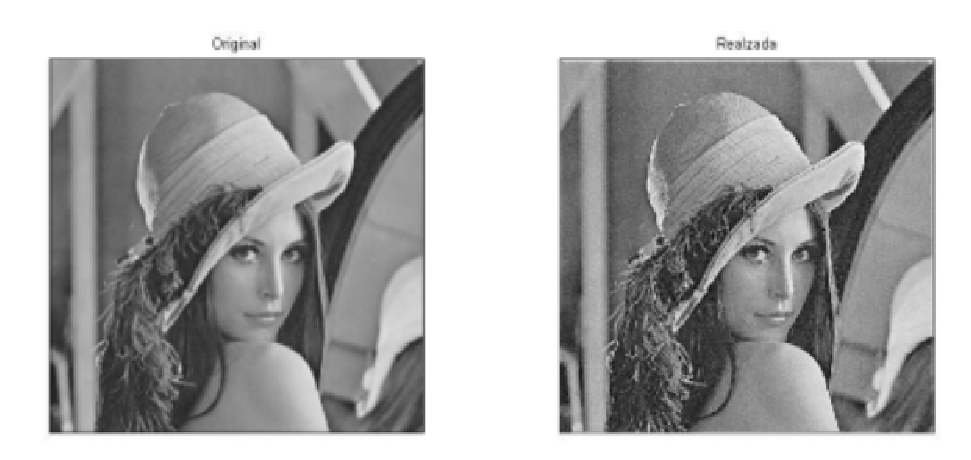
\includegraphics[width=0.5\textwidth]{realce_bordes}
\end{center}
\begin{center}
\caption{\small{Realce de una Imagen}}
{\small{\cite{elizondo2002fundamentos}}}
\end{center}
\end{figure}
\vskip 0.3cm


\item[4)] Amplificación/Reducción de imágenes 
\vskip 0.3cm
La ampliación o reducción de una imagen consiste en ampliar o disminuir la cantidad de pixeles de la matriz de la imagen , este proceso se realiza obteniendo el promedio de los vecinos del pixel para pintar los nuevos pixeles si es para amplificar y cuando se reduce ese promedio servirá para solo quedarse con un pixel de la vecindad. \par

\vskip 0.3cm



\end{enumerate}

\subsubsection{Procesamiento de Imágenes}
\begin{enumerate}
\item[1)] Binarización de una imagen
La binarización de una imagen consiste en comparar los niveles de gris presentes en la imagen con un valor (umbral) predeterminado. Si el nivel de gris de la imagen es menor que el umbral predeterminado, se le asigna al píxel de la imagen binarizada el valor 0 (negro), y si es mayor, se le asigna un 1 (blanco). De esta forma se obtiene una imagen en blanco y negro. Generalmente se utiliza un umbral de 128 si se trabaja con 255 niveles de gris, pero en algunas aplicaciones se requiere de otro umbral. En la figura 6 se muestra un ejemplo de imagen binarizada.\citep{elizondo2002fundamentos} \par 
\begin{figure}[ht]
\begin{center}
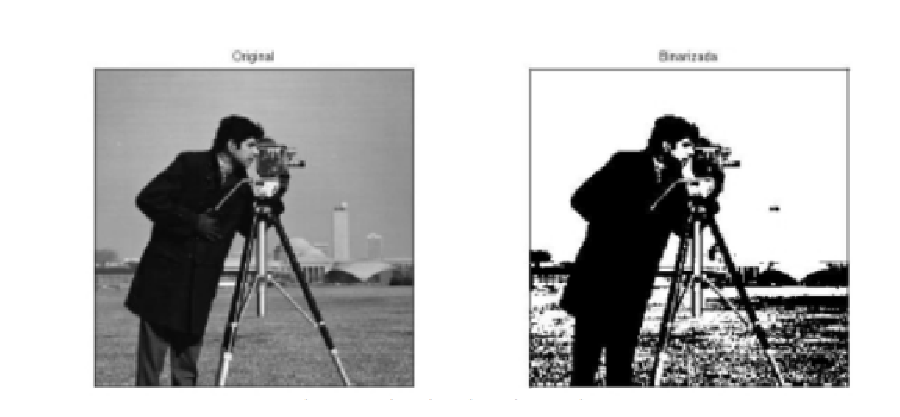
\includegraphics[width=0.5\textwidth]{binarizacion}
\end{center}
\begin{center}
\caption{\small{Binarización de una imagen}}
{\small{\cite{elizondo2002fundamentos}}}
\end{center}
\end{figure}
\vskip 4cm
\end{enumerate}

\subsubsection{Redes Neuronales}
\begin{enumerate}
\item[1)] Definición de Red Neuronal
\vskip 0.3cm
Según \cite{regueiro} una Definición general de una RNA (Red Neuronal Artificial) es la de un sistema de procesamiento de información compuesto por un gran número de elementos de procesamientos (EP), Profusamente conectados entre sí a través de canales de comunicación normalmente unidireccionales, que operan sobre información local (interna y externa).Sin embargo esta definición es muy vaga, ya que abarca no solo alas RNA sino también a los computadores masivamente paralelos.\par
\citep{regueiro} Una definición las específica y propia, sin embargo, debe de hacer hincapié a aspectos como la motivación, orientación y auto organización, entre otros. La motivación de su diseño distingue a las RNA de otras técnicas computacionales. Las RNA son dispositivos de procesamiento, tanto un algoritmo como un dispositivo real, cuya realización ha sido motivada, aunque sea de lejos, por el diseño y funcionalidad de cerebro humano y los componentes del mismo. Esta es su principal razón de ser y la idea subyacente que da coherencia al campo que se da en dominar RNA. Esta es también la causa de que mucha terminología usada en RNA provenga en realidad de las ciencias de lo natural.\par
Para \cite{hilera_gonzales} “Un sistema de computación hecho por un gran número de elementos simples, elementos de proceso altamente interconectados, los cuales procesan información por medio de su estado dinámico como respuesta a entradas externas”.\par
También en su libro dice que “Redes neuronales artificiales son redes interconectadas masivamente en paralelo de elementos simples (usualmente adaptativos) y con organización jerárquica, las cuales intentan interactuar con los objetos del mundo real del mismo modo que lo hace el sistema nervioso biológico”.\par
\vskip 5cm


\item[2)] Estructura Básica de la red
\vskip 0.1cm

\begin{figure}[ht]
\begin{center}
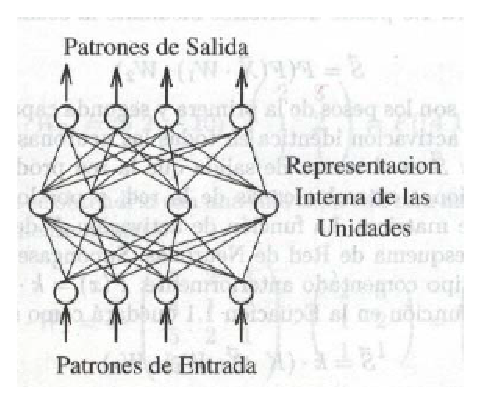
\includegraphics[width=0.7\textwidth]{estructurabasica}
\end{center}
\begin{center}
\caption{\small{Esquema de una red de tres capas totalmente interconectadas}}
{\small{Fuente : \cite{Isasi}}}
\end{center}
\end{figure}

La figura 7 se trata de una estructura típica de implementación de paradigma conocido como RETROPROGACION, la cual será descrita más adelante. El primer nivel lo constituyen las células de entrada; estas unidades reciben los valores de unos patrones representados como vectores que sirven de entrada a la red. Luego vemos una seria de capas intermedias, llamas ocultas, cuyas unidades responden a rasgos particulares que pueden aparecer en los patrones de entrada. Puede haber uno o varios niveles ocultos. El último nivel es el de salida. La salida de estas unidades sirve como salida de toda la red.\par
Cada interconexión entre unidades de proceso actúa como una ruta de comunicación: a través de etas interconexiones viajan valores numéricos de una célula a otra. Estos valores son evaluados por los pesos de las conexiones. Los pesos de las conexiones se ajustan durante la fase de aprendizaje para producir una red de neuronas artificial final. \citep{Isasi}.\par

\vskip 0.3cm

\item[3)] Modelo Neuronal
\vskip 0.3cm
Según \cite{serrano} en todo modelo artificial de neurona se tiene cuatro elementos básicos(Ver Figura 8):
\begin{enumerate}
\item[a)] Un conjunto de conexiones, pesos o sinapsis que determinan el comportamiento de la neurona. Estas conexiones pueden ser excitadoras (presentan un signo positivo), o inhibidoras (conexiones negativas).\par
\item[b)] Un sumador que se encarga de sumar todas las entradas multiplicadas por las respectivas sinapsis.
\item[c)] Una función de activación no lineal para limitar la amplitud de la salida de la Neurona.
\item[d)] Un umbral exterior que determina el umbral por encima de la cual la neurona se activa.
\end{enumerate}

\begin{figure}[ht]
\begin{center}
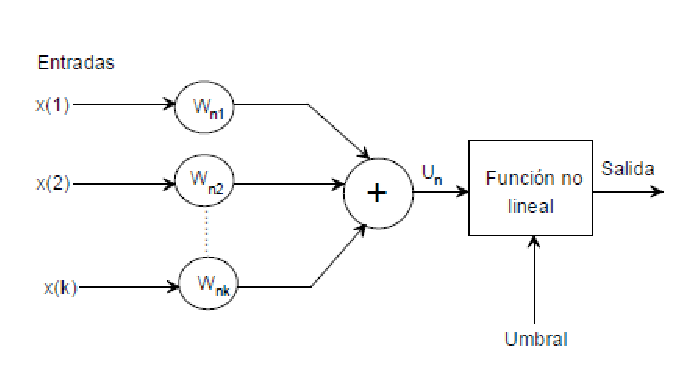
\includegraphics[width=0.7\textwidth]{modelo_neuronal}
\end{center}
\begin{center}
\vskip -0.5cm
\caption{\small{Modelo Neuronal}}
{\small{Fuente : \cite{serrano}}}
\end{center}
\end{figure}

\vskip 4cm

\item[4)] Arquitecturas Neuronales
\vskip 0.3cm
\begin{enumerate}

\item[a)] Según número de capas:\par
- Redes Neuronales Monocapa:Se corresponde con la red neuronal más sencilla ya que se tiene una capa de neuronas que proyectan las entradas a una capa de neuronas de salida donde se realizan diferentes cálculos. La capa de entrada, por no realizar ningún calculo, no se cuenta de ahí el nombre de redes neuronales con una sola capa.(Ver Figura 9)\par
\begin{figure}[ht]
\begin{center}
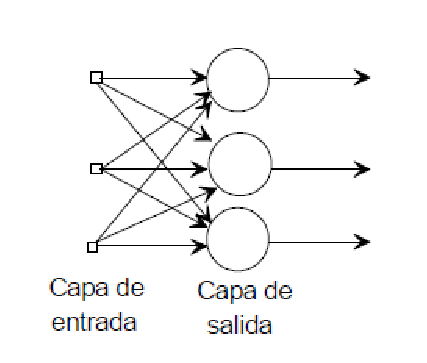
\includegraphics[width=0.2\textwidth]{rna_monocapa}
\end{center}
\begin{center}
\caption{\small{Red Neuronal Monocapa }}
{\small{Fuente : \cite{serrano}}}
\end{center}
\end{figure}
\vskip 4cm
- Redes Neuronales Multicapa:Es una generalización de la anterior existiendo un conjunto de capas intermedias entre la entrada y la salida (capas ocultas). Este tipo de red puede estar total o parcialmente conectada.(Ver Figura 10)\par
\begin{figure}[ht]
\begin{center}
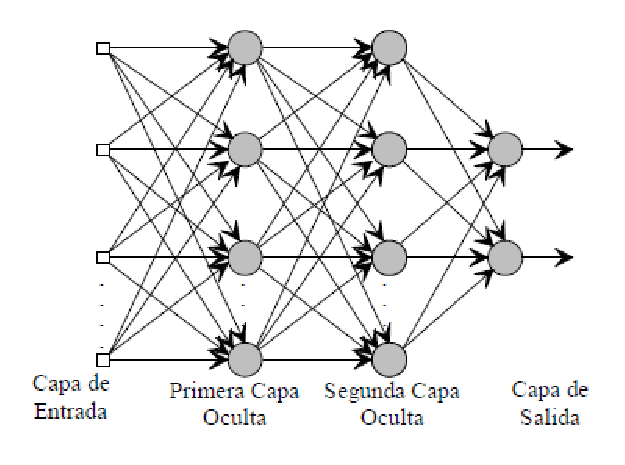
\includegraphics[width=0.3\textwidth]{rna_multicapa}
\end{center}
\begin{center}
\caption{\small{Red Neuronal Multicapa}}
{\small{Fuente : \cite{serrano}}}
\end{center}
\end{figure}
\item[b)] Según tipo de conexiones:\par
- Redes Neuronales No Recurrentes:En esta red la propagación de las señales se produce en un sentido solamente, no existiendo la posibilidad de realimentaciones. Lógicamente estas estructuras no tienen memoria.\par
- Redes Neuronales Recurrentes:esta red viene caracterizada por la existencia de lazos de realimentación. Estos lazos pueden ser entre neuronas de diferentes capas, neuronas de la misma capa o, más sencillamente, entre una misma neurona. Esta estructura recurrente la hace especialmente adecuada para estudiar la dinámica de sistemas no lineales.(Ver Figura 11)\par
\begin{figure}[ht]
\begin{center}
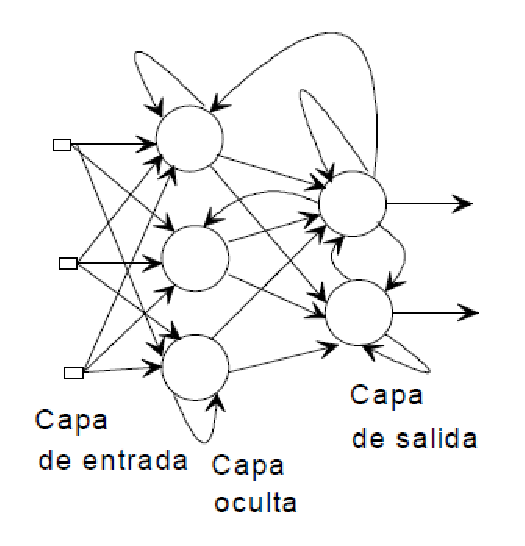
\includegraphics[width=0.3\textwidth]{rna_recurrente}
\end{center}
\begin{center}
\caption{\small{Red neuronal recurrente}}
{\small{Fuente : \cite{serrano}}}
\end{center}
\end{figure}
\vskip 6cm
\item[c)] Según grado de conexión:\par
- Redes Neuronales Totalmente Conectadas:En este caso todas las neuronas de una capa se encuentran conectadas con las de la capa siguiente (redes no recurrentes) o con las de la anterior (redes recurrentes).\par
- Redes Neuronales Parcialmente Conectadas:En este caso no se da la conexión total entre neuronas de diferentes capas.\par


\end{enumerate}


\item[5)] La Neurona,Modelo Biológico
\vskip 0.3cm
\citep{hilera_gonzales} Una neurona es una célula viva y, como tal, contiene los mismos elementos que forman parte de todas las células biológicas. Además contienen elementos característicos que las diferencian. En general, una neurona consta de un cuerpo celular más o menos esférico, de 5 a 10 micras de diámetro, del que salen una rama principal, el axón, y varias ramas más cortas llamadas dendritas. A su vez el axón puede producir ramas entorno a su punto de arranque y, con frecuencia, se ramifica extensamente cerca de su extremo.(Ver Figura 12)\par

\begin{figure}[ht]
\begin{center}
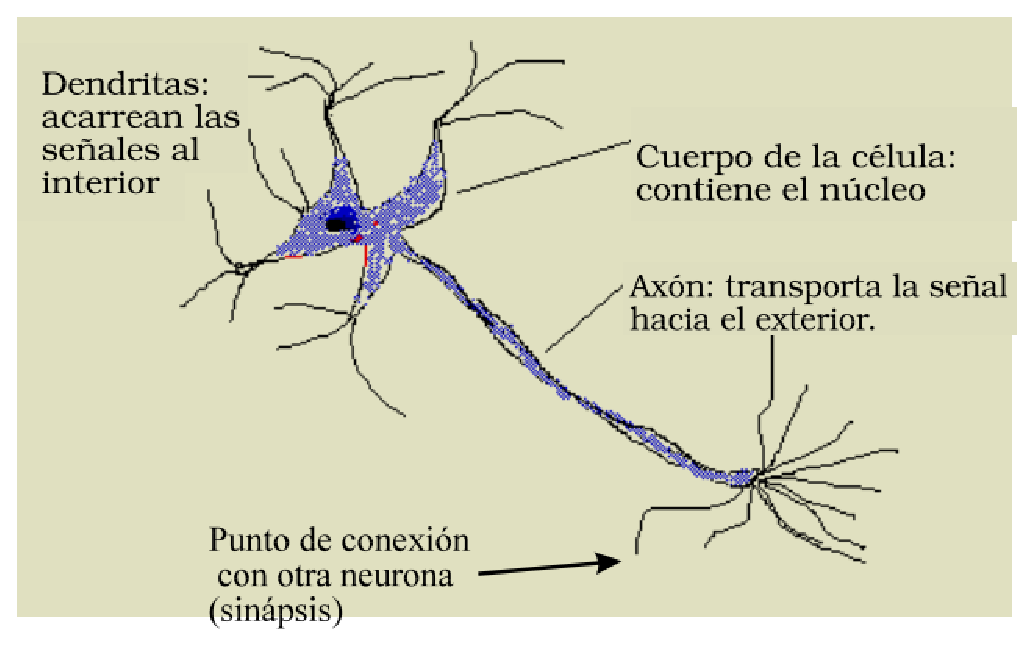
\includegraphics[width=0.3\textwidth]{neurona}
\end{center}
\begin{center}
\caption{\small{Forma General de Una Neurona}}
{\small{Fuente : \cite{hilera_gonzales}}}
\end{center}
\end{figure}

\vskip 7cm

\item[6)] La Neurona Artificial
\vskip 0.3cm
\citep{Isasi} La neurona artificial, célula o autómata, es un elemento que posee un estado interno, llamado nivel de activación, y recibe señales que le permiten, en su caso, cambiar de estado.\par
Se denomina S al conjunto de estados posibles de una neurona. S podrá ser por ejemplo, S= {0,1}, siendo 0 el estado inactivo y 1 el activo. S también podrá tomar un mayor número de valores, S = {0, 1, 2, 3,…, n} para representar, por ejemplo, una imagen con n+1 niveles de gris, p incluso un intervalo continuo de valores, por ejemplo S = [0,1].\par
Las neuronas poseen una función que les permite cambiar de nivel de activación a partir de las señales que recibe; a ducha función se la denomina función de transición de estado o función de activación. Las señales que recibe cada neurona pueden provenir del exterior o de las neuronas las cuales esta conecta.\par
El nivel de activación de una célula depende de las entradas recibidas y de los valores sinápticos, pero no de anteriores valores de estados de activación. Para calcular el estado de activación se ha de calcular en primer lugar la entrada total a la célula, Ei. Este valor se calcula como la suma de todas las entradas ponderadas por ciertos valores.\par
\begin{figure}[ht]
\begin{center}
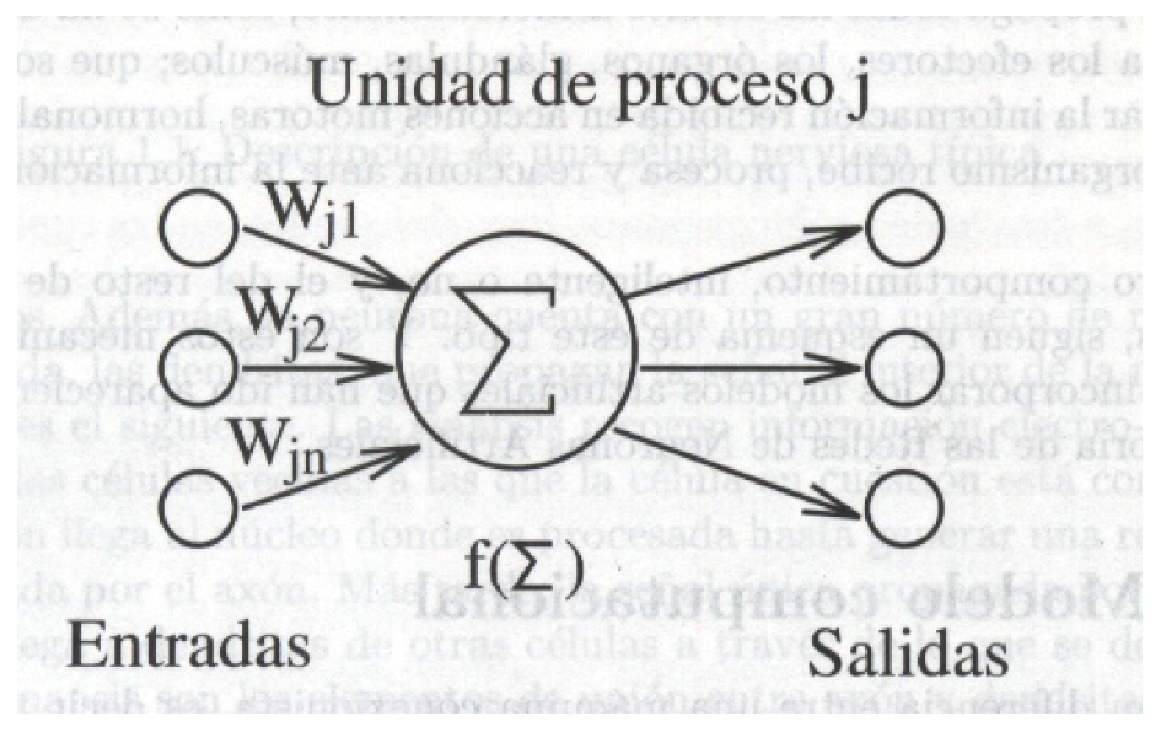
\includegraphics[width=0.7\textwidth]{neurona_artificial}
\end{center}
\begin{center}
\caption{\small{Esquema de una unidad de Proceso típica}}
{\small{Fuente : \cite{Isasi}}}
\end{center}
\end{figure}
La figura 13 muestra un modelo que representa esta idea. Aquí un grupo de entradas x1, x2, x3,…, Xn son introducidas en una neurona artificial.Estas entradas, definidas por un vector $\overline{X}$, corresponden a las señales de la sinapsis de una neurona biológica. Cada señal se multiplica por un peso asociado w1, w2,…, wn antes de ser aplicado el sumatorio etiquetado por $ \sigma $. Cada peso corresponde a la fuerza de una conexión sináptica, es decir el nivel de concentración ionica de la sinapsis, y se representa por un vector $\overline{W}$ .\par
El sumatorio, que corresponde al cuerpo de la neurona, suma todas las entradas ponderadas algebraicamente, produciendo una salida que se denomica E, asi:
$$E= x1w1+x2w2+ … + xnwn$$
Las señales E son procesadas además por una función llamada función de activación o de salida $\mathcal{F}$, que produce la señal de salida de la neurona S.\par

\vskip 0.3cm


\item[7)] Perceptrón
\vskip 0.3cm
\citep{serrano} La primera estructura neuronal a estudiar es la más sencilla y la que, desde un punto de vista histórico, apareció la primera. Esta estructura se usó en problemas de clasificación y tiene el siguiente esquema:\par
\begin{figure}[ht]
\begin{center}
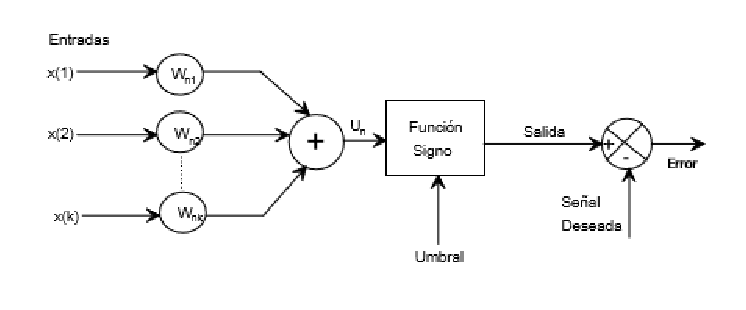
\includegraphics[width=0.7\textwidth]{perceptron}
\end{center}
\begin{center}
\caption{\small{Esquema del Perceptrón}}
{\small{Fuente : \cite{serrano}}}
\end{center}
\end{figure}
El funcionamiento del perceptrón se basa en comparar la salida del sistema con una señal deseada (que es la que debería dar el sistema). De la estructura, más concretamente de la función de activación, se deduce que este elemento es un clasificador binario ya que puede determinar la pertenencia por parte del vector de entrada a dos clases diferentes.\par
El algoritmo que sigue este sistema es de tipo supervisado ya que necesitamos un elemento exterior que plantee la clase de pertenencia del elemento de entrada.\par
El procedimiento de aprendizaje comienza por la inicialización aleatoria de los pesos, para, posteriormente, irlos ajustando conforme la red se equivoca en la asignación de clase al vector de entrada presente en ese momento.\par

\vskip 0.3cm


\item[8)] Aprendizaje del Perceptrón
\vskip 0.3cm
Según \cite{serrano} :\par
1.	Inicialización de los pesos.\par
2.	Determinación de la salida:\par
$$y= \sum_{k=1}^N W_n^k.X_n^k$$
3.	Comparación con el umbral:\par
$$u=y-umbral$$
4.	Aplicación de la función signo: \par
$$0=signo(u)$$
5.	Comparación con la señal deseada.\par
6.	Actualización de los coeficientes si existe error.\par
$$w_k = w_k + \alpha.(d-o)x_k$$
El funcionamiento del perceptrón como clasificador se basa en la función signo, es decir:\par
$$sign(o)=\left\{\begin{matrix}
+1 &si  & o\geq 0\\ 
 0& si & o<0
\end{matrix}\right.
$$
Modificamos el rango de la función $signo(\pm 1)$( en el caso más común) porque nos resulta más conveniente.\par
De la anterior expresión, se deduce que la frontera de decisión se toma para o=0. Tomemos un caso simple en el que tendremos dos entradas, x1 y x2, para comprender que significa esto. Si la salida, tras aplicar la función signo, vale cero significa que:\par
$$o=w_0+w_1.x_1+w_2.x_2$$
Despejando X2 en la anterior ecuación:\par
$$x_2=-\frac{w_0}{w_2}-\frac{w_1}{w_2}.x_1$$
Si nos fijamos, la anterior expresión es la ecuación de una recta en el espacio definido por los patrones de entrada; este es; la superficie de separación entre clases diferentes en una recta. De aquí se deduce que se tendrá una clasificación perfecta si los patrones son linealmente separables.\par

\vskip 0.3cm

\item[9)] Perceptrón Multicapa
\vskip 0.3cm

- Definición:
\vskip 0.3cm
El perceptrón multicapa es la red neuronal artificial más conocida y con un mayor número de aplicación. Su historia comienza en 1958 cuando Rosenblatt publica los primeros trabajos sobre un modelo neuronal y su algoritmo de aprendizaje que se llama perceptrón.\par
El perceptrón está formado por una única neurona, por lo que su utilización está limitada a la clasificación de patrones en dos clases. Si se expande esta cala de salida con más de una neurona se podrán clasificar más de dos clases, aunque con la limitación demostrada por Minsky y Papert en 1969 de que estas clases deben ser, linealmente separables. Esta limitación es bastante problemática porque imposibilita al perceptrón para resolver un problema tan sencillo como el de la función lógica XOR de 2 entradas cuya tabla de verdad es la mostrada a continuación:\par
\vskip 2cm
\begin{figure}[ht]
\begin{center}
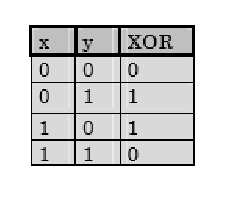
\includegraphics[width=0.2\textwidth]{tabla_xor}
\end{center}
\begin{center}
\caption{\small{Tabla de verdad XOR}}
{\small{Fuente : \cite{serrano}}}
\end{center}
\end{figure}

La figura 16 muestra que las dos clases son no linealmente separables representándose los ceros por círculos y los unos por cuadrados.\par
\begin{figure}[ht]
\begin{center}
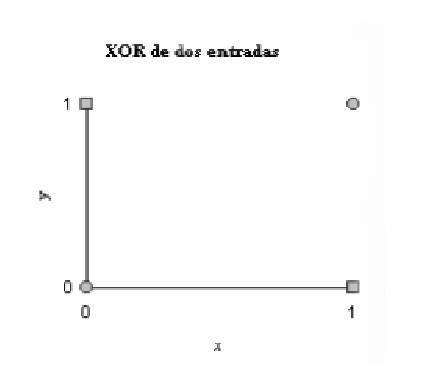
\includegraphics[width=0.3\textwidth]{linealmente_separables}
\end{center}
\begin{center}
\caption{\small{Función lógica XOR de dos entradas}}
{\small{Fuente : \cite{serrano}}}
\end{center}
\end{figure}

La separación de clases no linealmente separables se consigue introduciendo una capa de neuronas entre la salida y la entrada. Aparece entonces el problema de asignar un “error” durante el proceso de aprendizaje a estas neuronas; este problema es conocido en la teoría de los sistemas conexionistas como el problema de la asignación de crédito citep/{serrano}. \par 

- Arquitectura:
\vskip 0.3cm
La arquitectura del perceptrón multicapa se caracteriza porque tiene sus neuronas agrupadas en capas de diferentes niveles, cada una de las capas está formada por un conjunto de neuronas y se distinguen tres tipos de capas diferentes: la capa de entrada, las capas ocultas y la capa de salida. \citep{Isasi}
\begin{figure}[ht]
\begin{center}
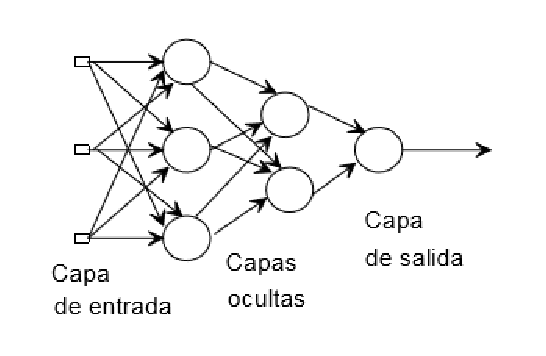
\includegraphics[width=0.3\textwidth]{perceptron_multicapa}
\end{center}
\begin{center}
\caption{\small{Estructura de un perceptrón multicapa}}
{\small{Fuente : \cite{serrano}}}
\end{center}
\end{figure}
\vskip 0.3cm
Según \cite{serrano} las cuatro características fundamentales de esta arquitectura son las siguientes:\par
•	Se trata de una estructura altamente no lineal.\par
•	Presenta tolerancia a fallos.\par
•	El sistema es capaz de establecer una relación entre dos conjuntos de datos.\par
•	Existe la posibilidad de realizar una implementación hardware.\par
De la figura 17 se desprende que es una estructura formada por nodos o neuronas que propagan la señal hacia la salida. Las conexiones entre neuronas se denominan pesos sinápticos, que son optimizados por el algoritmo de aprendizaje.\par
La propagación se realiza de manera que cada neurona hace una combinación lineal de la señal procedente de las neuronas de la capa anterior, siendo los coeficientes de esta combinación los pesos sinápticos. A continuación, se aplica una función de activación no lineal. Estas neuronas se conocen como neuronas no lineales y aseguran la alta no linealidad en MLP.\par


\vskip 0.3cm

\item[10)] Algoritmo BackPropagation
\vskip 0.3cm
El proceso de back propagation consiste en dos pasadas a través de las diferentes capas de la red. Una pasada hacia adelante y una pasada hacia atrás. En la pasada hacia adelante, se aplica en la capa de entrada un patrón o vector de entrada, este propaga su efecto a través de las diferentes capas y como consecuencia produce un vector de salida. Durante este proceso, los pesos sinápticos de la red son fijos y no se modifican.\par
Durante la pasada hacia atrás en cambio. Los pesos su se modifican de acuerdo con la regla de corrección del error. La señal de salida real se compara con la señal deseada y como resultado se obtiene una señal de error, que se propaga en dirección contraria a través de la red modificando los pesos, de forma que, al volver a pasar el vector de entrada hacia adelante, la respuesta obtenida se asemeje más a la salida deseada .\citep{emiliano}\par
El desarrollo del algoritmo back propagation proporciona un método eficiente para entrenar este tipo de redes. Aunque no es capaz de resolver todos los problemas, se han demostrado como el mejor de todos. Su importancia está en su capacidad de auto adaptar los pesos de las neuronas intermedias para aprender la relación que existe entre el conjunto de vectores a patrones de entrada y su correspondiente salida, y poder aplicar esa relación después del entrenamiento a nuevos vectores de entrada imperfectos o con ruido. Esta capacidad se conoce como generalización. La red debe encontrar una representación interna que le permita generar las salidas deseadas durante la etapa de entrenamiento t posteriormente durante el funcionamiento ser capaz de generar salidas para entradas que no le fueron mostradas durante el aprendizaje pero que se asemejen a algunas de las que si fueron mostradas.\par

\vskip 0.3cm

\end{enumerate}


\subsection{Descripción de la realidad}


Según \cite{ayunque}, en los últimos diez años (2004 - 2015) se han reportado 1, 041,704 accidentes de tránsito, los principales factores que la generan son, el exceso de velocidad. Estas cifras y la probabilidad que suceda una tragedia al volante pueden reducirse significativamente si se mejora el monitoreo de vehículos.\par 
El autor propone “la ciudad del futuro”, es decir inteligente: con la capacidad de encontrar personas desaparecidas, reconocer zonas donde se vive con más pobreza para mejorar la distribución de bienes y reconocer actos criminales como violación de señales de tránsito. 
De los 1, 041, 704 accidentes de tránsito, 598, 912 son heridos y 38,567 son muertos, estas cifras pueden ser mayores puesto a que solo reflejan la situación de lesionados o fallecidos que hay  en el lugar mismo del accidente, si unos días después, una víctima queda incapacitada o fallece, no se incluyen en las estadísticas.\par
EL beneficio de reconocer señales de tránsito se puede verificar si los vehículos cumplen o incumplen la señal, de cometer alguna infracción, se puede enviar alertas a los conductores, y emitir multas respectivas.\par
Según  \cite{ayunque} El tráfico y la congestión vehicular es un problema grave en varias ciudades del mundo, sobre todo en la ciudad de lima, la cual se muestra en la Figura 18. Y que es considerada una de las peores ciudades Sudamérica para conducir.\par


\begin{figure}[ht]
\begin{center}
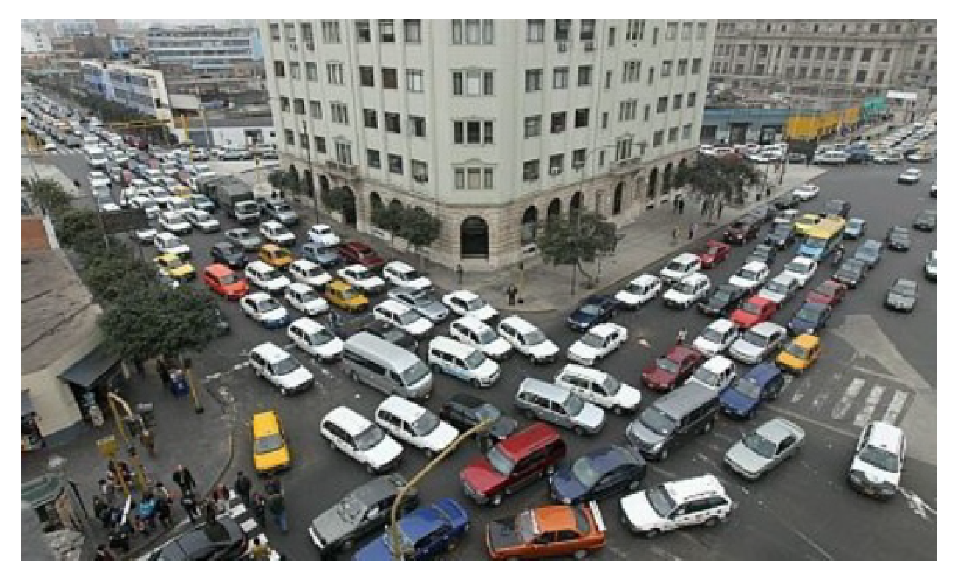
\includegraphics[width=0.7\textwidth]{problema1}
\end{center}
\begin{center}
\vskip -0.5cm
\caption{\small{Caos y congestión vehicular en Lima.}}
{\small{Fuente : \cite{ayunque}}}
\end{center}
\end{figure}



Si se quiere regularizar el tráfico se requiere la intervención humana, como un policía de tránsito; sin embargo, la policía nunca se va a dar de abasto controlando a todos los autos, tampoco tiene las herramientas para ello.
Monitorear que se están respetando las señales de tránsito es un problema general que se requiere de varias soluciones, y la clasificación en el que se determina qué tipo de señal de transito es el identificado (Figura 19).\par


\begin{figure}[ht]
\begin{center}
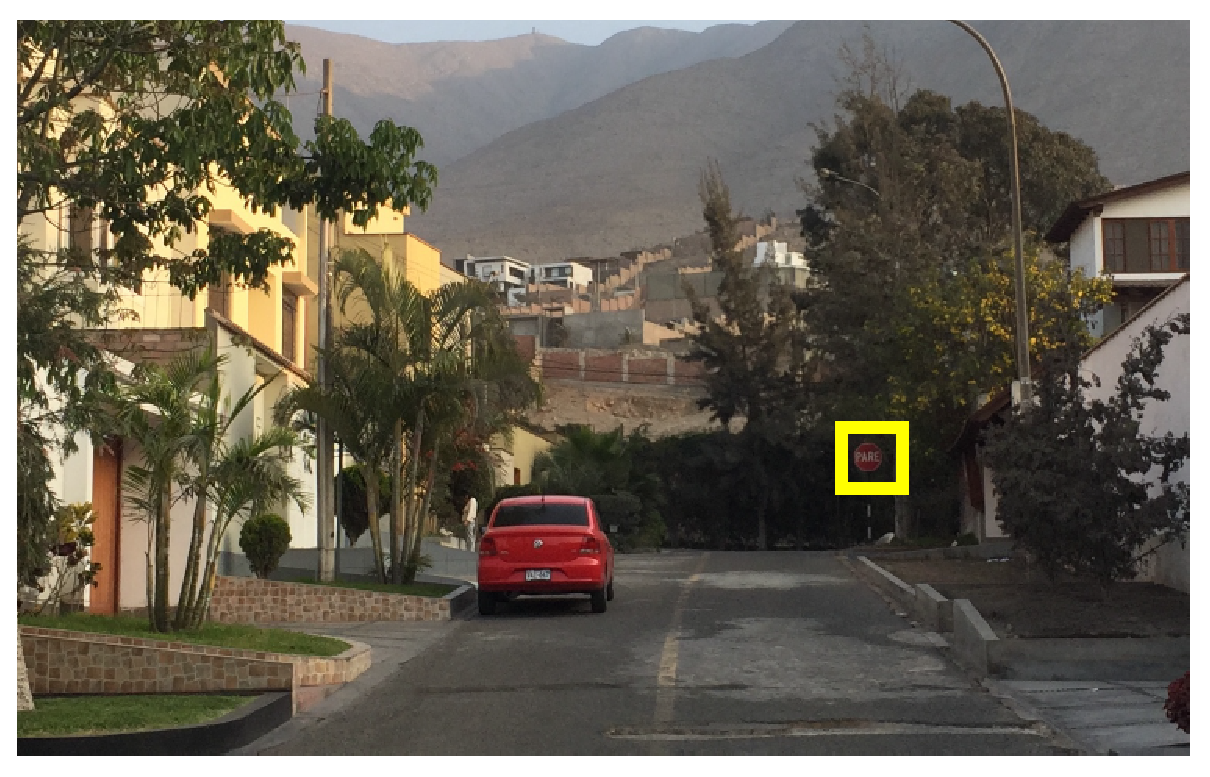
\includegraphics[width=0.7\textwidth]{problema2}
\end{center}
\begin{center}
\vskip -0.5cm
\caption{\small{Detección de una señal de tránsito}}
{\small{Fuente : \cite{ayunque}}}
\end{center}
\end{figure}


Por lo expuesto se propone la implementación de un software el cual consiste en reconocer y clasificar señales de tránsito . La implementación de dicho software esta compuesta de dos etapas bien marcadas :la primera etapa consiste en el pre procesamiento y procesamiento de la imagen , es decir , preparar la imagen para obtener un descriptor de características , para la realización de esta etapa se utilizo segmentación , el algoritmo surf y  métodos de filtrado para la eliminación del ruido.
La segunda etapa es la creación y entrenamiento de las redes neuronales perceptron multicapa (mediante el algoritmo back propagation) que recibirán como entrada el descriptor de características y devolverán la clasificación a la que pertenece dicha señal de tránsito entrante.\par
\vskip 0.5cm


El funcionamiento del software se realiza primero tomando foto de la imagen con una cámara en tiempo real,luego se realiza la primera etapa de procesamiento de la imagen , seguidamente  el descriptor de características obtenido es introducido como entrada a las redes neuronales perceptron multicapa para su clasificación y por ultimo el software devuelve como salida el tipo de señal de tránsito que es (Ver Figura 20).\par

\begin{figure}[ht]
\begin{center}
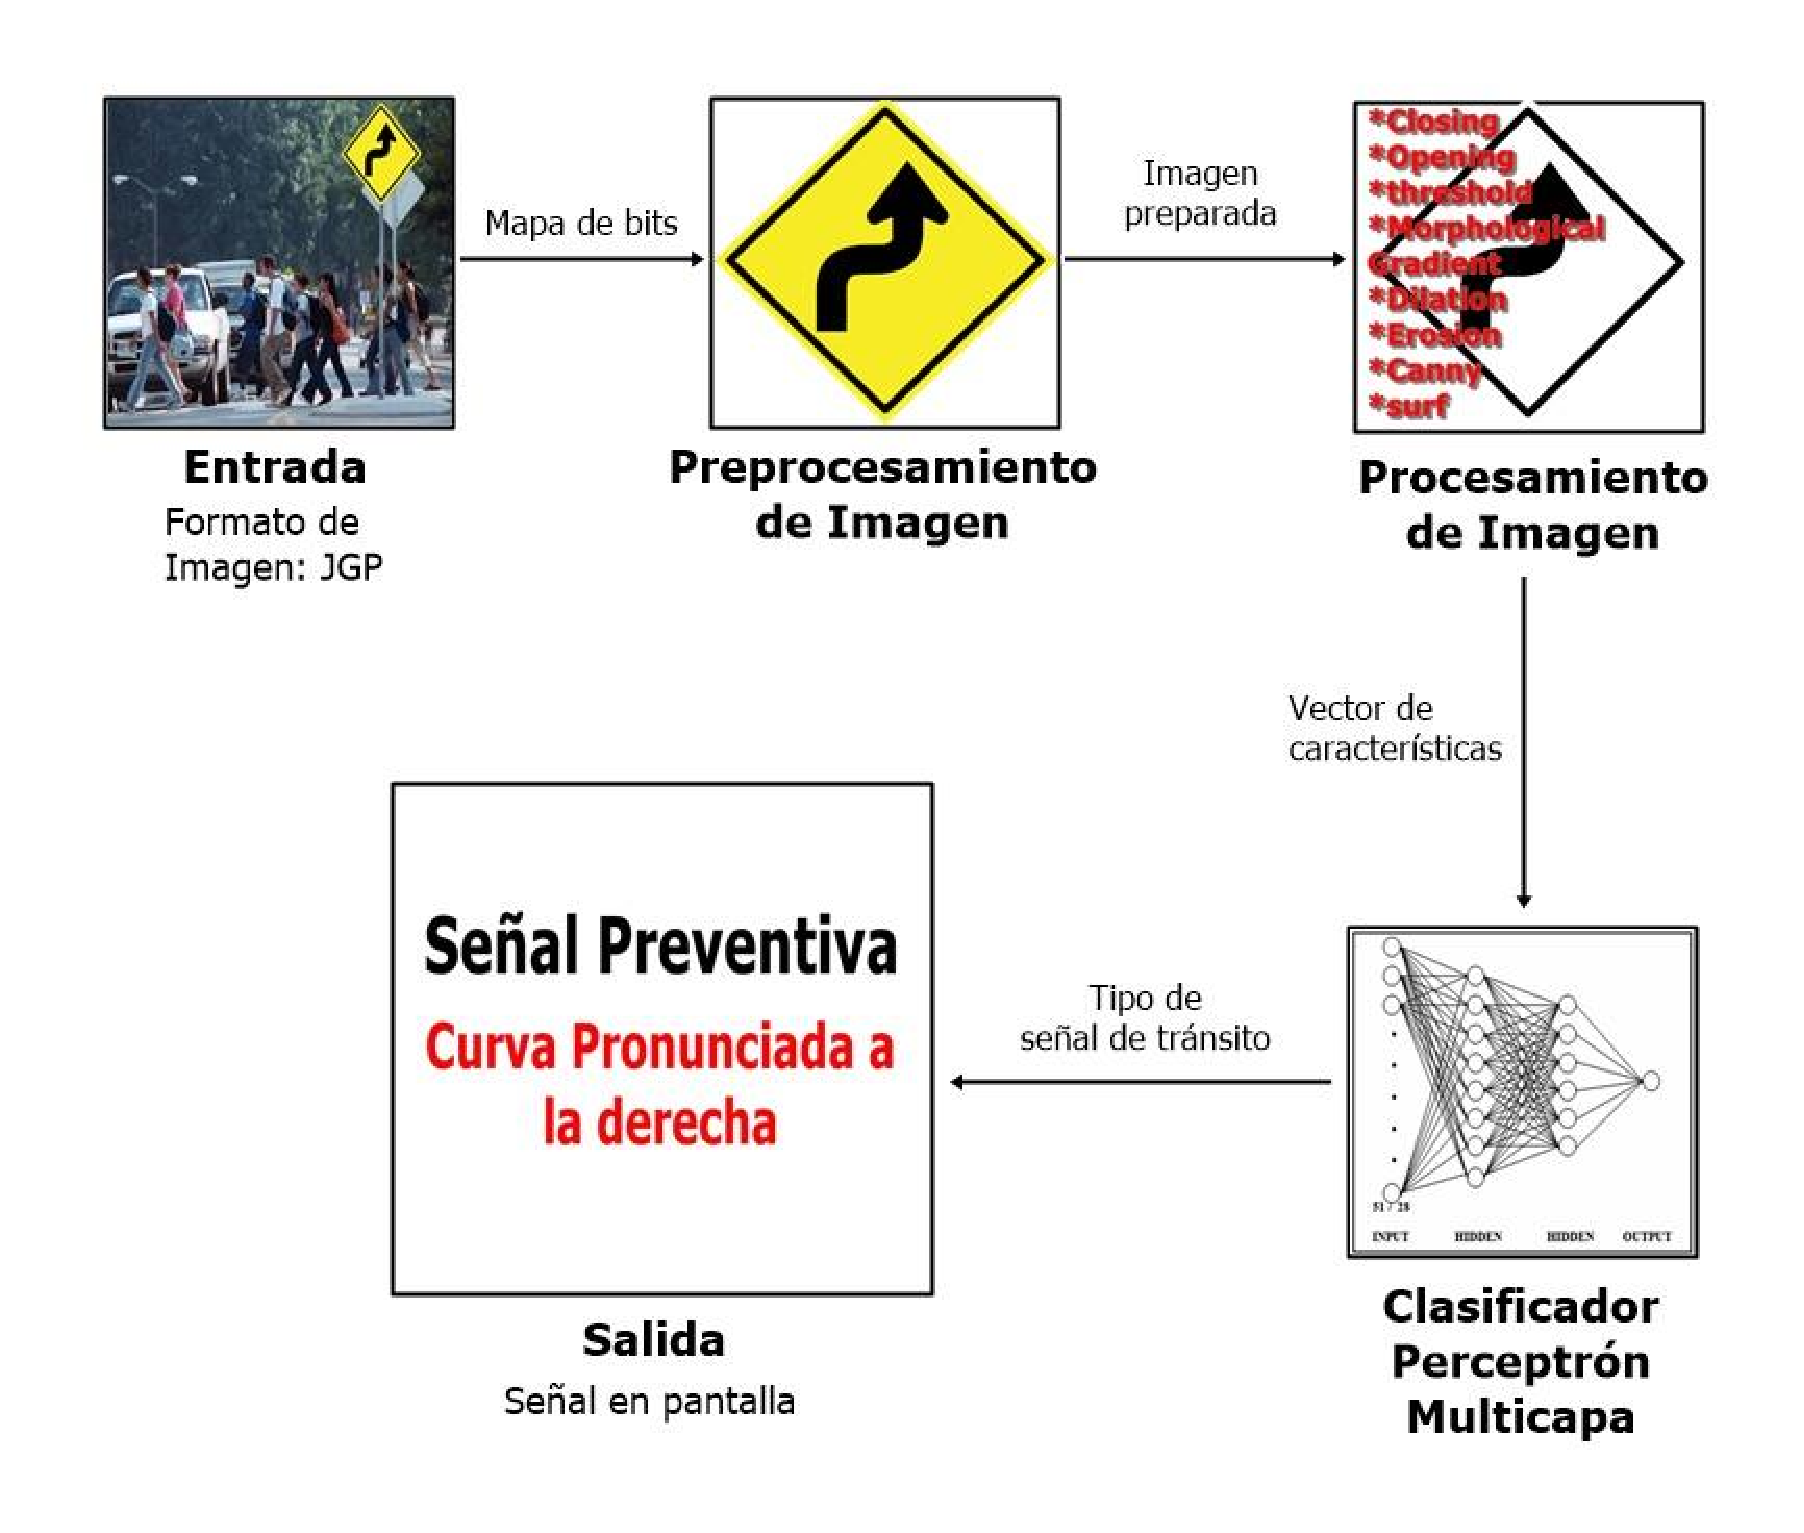
\includegraphics[width=0.7\textwidth]{funcionamiento}
\end{center}
\begin{center}
\vskip -0.5cm
\caption{\small{Diagrama de bloques del Funcionamiento de nuestro software.}}
{\small{Elaboración propia}}
\end{center}
\end{figure}

\newpage
\subsection{Justificación}
Justificación Académica :
\vskip 0.2cm
El presente trabajo se realiza con el fin de aplicar los conocimientos adquiridos en el curso de Inteligencia Artificial tratando de profundizar mas en el tema de la red neuronal perceptrón multicapa implementando 3 redes para un problema complejo como lo es el reconocimiento de señales de tránsito. Profundizaremos en tema del diseño y el entrenamiento de las redes neuronales, tipos de RNA(en cuanto a cantidad de neuronas por capa) y cual es el margen de error de cada una de ellas.\par
\vskip 0.2cm
Se realiza con el fin de analizar y aplicar los diferentes tipos de procesamientos de imágenes que existe para conocer a fondo la utilidad de cada uno de ellos.\par
\vskip 0.4cm
Justificación Social: 
\vskip 0.2cm
Se realiza con el propósito de reducir los accidentes de tránsito comunes y muerte de personas a causa de no respetar las señales de tránsito implementando cámaras de vigilancia que utilicen nuestro sistema de clasificación para monitorear si se respetan las señales de tránsito o para implementar programas de asistencia a los conductores , los cuales brinden al usuario un aviso que una señal fue detectada y de que tipo de señal se trata.\par
\vskip 0.2cm
Se realiza con el propósito de dejar para el futuro un sistema que servirá de soporte a futuros proyectos como es el enrutamiento de vehículos automáticos, es decir, sin la necesidad de una persona a cargo del volante.\par
\vskip 0.4cm

\subsection{Problema}
¿Como podemos reconocer automáticamente las señales de tránsito?

\subsection{Hipótesis}
La elaboración de un software utilizando procesamiento de imágenes
y el diseño de una red perceptrón multicapa permite reconocer automáticamente señales de tránsito.

\subsection{Objetivos}

\subsubsection{Objetivos generales}
Elaborar un software utilizando procesamiento de imágenes y diseñar una red perceptrón multicapa para reconocer automáticamente señales de tránsito.
\vskip 0.3cm

\subsubsection{Objetivos específicos}
\vskip 0.2cm
\begin{enumerate}
\item[a)] Analizar diferentes algoritmos de pre procesamiento y procesamiento de imágenes.
\item[b)] Diseñar la red neuronal perceptrón multicapa que servirá para la clasificación de las imágenes capturadas.
\item[c)] Entrenar la red neuronal mediante el algoritmo Backpropagation para  ajustar que las salidas generadas de acuerdo a las características de entrada sea la correcta.
\item[d)] Realizar pruebas con las imágenes obtenidas de la cámara en tiempo real.

\end{enumerate}



\subsection{Metodología de trabajo}
\vskip 0.1cm
Para llegar a los objetivos propuestos, el desarrollo de la investigación comprendió las siguientes etapas de trabajo a saber:\par
\begin{enumerate}
\item[a)] Adquisición de las imágenes
\vskip 0.1cm
Las imágenes de las señales de tránsito serán tomadas en tiempo real por una cámara digital .
\item[b)] Pre procesamiento de Imágenes
\vskip 0.1cm
Aplicamos el método de segmentación , el algoritmo surf para obtener solo la señal de tránsito de la imagen de entrada, aplicamos algoritmos de filtrado para eliminar el ruido ,corregimos la orientación de la imagen y aplicamos un algoritmo de reducción o extension de imagen para tener la señal en un tamaño especifico.
\item[c)] Procesamiento de Imágenes
\vskip 0.1cm
Aplicamos el algoritmo de binarización y umbralización para obtener la imagen en blanco y negro y obtenemos la matriz de pixeles de esa imagen resultante donde cada pixel será la entrada a la red neuronal .\par
\item[d)] Diseño de las 3 redes neuronales perceptron multicapa
\vskip 0.1cm
Teniendo las plantillas de las diferentes señales de transito analizaremos y diseñaremos las redes neuronales con la cantidad suficiente de neuronas en cada capa.
\item[e)] Entrenamiento de las 3 redes neuronales perceptron multicapa
\vskip 0.1cm
Las redes neuronales perceptron multicapa seran entrenadas con el algoritmo back propagation.
\item[f)] Implementación del software en el lenguaje de programación Java
\vskip 0.1cm
Utilizaremos la libreria Open CV y la integraremos con la red neuronal que obtenga menos porcentaje de error en el lenguaje de programación Java.
\item[g)] Prueba del software desarrollado
\vskip 0.1cm
Se realizará diferentes pruebas con la adquisición de nuevas imágenes en tiempo real 
\item[h)] Validación y conclusiones
\vskip 0.1cm
Para la validación utilizaremos una matriz de confusión.
   
\end{enumerate}
    
\subsubsection{Población y Muestra}
\begin{enumerate}
\item[•] Población de estudio
\vskip 0.1cm
La población esta conformada por los tipos de redes neuronales existentes.\par
\item[•] Muestra de estudio
\vskip 0.1cm
La muestra de estudio es no probabilística,corresponde a 3 redes neuronales perceptrón multicapa configuradas con diferentes capas y neuronas por capas.\par
\item[•] Variables de Investigación
\begin{enumerate}
\item[-] Variable Dependiente : 
Reconocimiento Automático de Señales de Tránsito
\item[-] Variable Independiente : 
Modelo de la Red Neuronal perceptrón Multicapa

\vskip 0.1cm

\end{enumerate}
\end{enumerate}

\subsubsection{Técnica de Recolección de Datos}
La técnica usada será la observación indirecta(medición) de los indicadores reportados por el software de reconocimiento automático de imágenes a través de la matriz de confusión.

\subsubsection{Análisis Estadístico}
La técnica usada es una matriz de confusión.La siguiente tabla indica su estructura.
\vskip 0.1cm
\begin{center}
\begin{tabular*}{5.8 cm}{||l | c | r||}
\hline
&Negativo&Positivo\\
\hline
Negativo&a&b\\
\hline
Positivo&c&d\\
\hline
\end{tabular*}
\end{center}

\vskip 0.1cm

Donde:\par
\vskip 0.1cm
\begin{enumerate}
\item[•] El positivo y negativo de la parte izquierda representa la realidad.\par
\item[•] El positivo y negativo de la parte superior representa la predicción.\par
\item[•] a es el número de predicciones correctas de que una instancia es negativa.\par
\item[•] b es el número de predicciones incorrectas de que una instancia es positiva.\par
\item[•] c es el número de predicciones incorrectas que una instancia negativa.\par
\item[•] d es el número de predicciones correctas que una instancia es positiva.\par
\end{enumerate}

Términos estándar :\par
\vskip 0.1cm
\begin{enumerate}

\item[•] La tasa de verdaderos positivos (TP) es la proporción de casos positivos que se identificaron correctamente, se calculó usando la ecuación:
\vskip 0.1cm
\begin{equation}
TP = \frac{d}{c + d}
\end{equation}
\vskip 0.1cm
\item[•] La tasa de falsos positivos (PF) es la proporción de casos negativos que se clasificaron incorrectamente como positivos, se calculó usando la ecuación:
vskip 0.1cm
\begin{equation}
FP = \frac{b}{a + b}
\end{equation}
\vskip 0.1cm
\item[•] La tasa de verdaderos negativos (TN) se define como la proporción de casos negativos que se clasificaron correctamente, se calculó usando la ecuación:
\vskip 0.1cm
\begin{equation}
TN = \frac{a}{a + b}
\end{equation}
\vskip 0.1cm
\item[•] La tasa de falsos negativos (FN) es la proporción de casos positivos que se clasificaron incorrectamente como negativos, se calculó usando la ecuación:
\vskip 0.1cm
\begin{equation}
FN = \frac{d}{b + d}
\end{equation}
\vskip 0.1cm
\item[•] La confiabilidad positiva  (CP) es la proporción de casos positivos predichos que fueron correctos, se calculó usando la ecuación:
\vskip 0.1cm
\begin{equation}
CP = \frac{d}{c + d}
\end{equation}
\vskip 0.1cm
\item[•] La confiabilidad negativa  (CN) es la proporción de casos negativos predichos que fueron correctos, se calculó usando la ecuación:
\vskip 0.1cm
\begin{equation}
CN = \frac{a}{a + c}
\end{equation}
\vskip 0.1cm
\item[•] La confiabilidad total  (CT) es el promedio de la CP y la CN, se calculó usando la ecuación:
\vskip 0.1cm
\begin{equation}
CT = \frac{CP + CN}{2}
\end{equation}
\vskip 0.1cm
\end{enumerate}


\newpage
\bibliography{Bibliografia}

\newpage

\vskip 5cm
\hspace{1.5cm}$\overline{Juan\hspace{.1cm} Polo\hspace{.1cm}Cosme}$ 
 \hspace{4.5cm} $\overline{Marlon\hspace{.1cm} Sanchez \hspace{.1cm}Chavez}$\\


\vskip 2cm
\begin{center}
$\overline{Jorge \hspace{.1cm} Gutierrez\hspace{.1cm}Gutierrez}$\\ $Asesor$
\end{center}


\end{document}

